\documentclass{beamer}
\usepackage[utf8]{inputenc}
\usepackage{pgfplots}
\pgfplotsset{compat=newest}
\usepackage{biblatex}
\bibliography{ref}
\usepackage{subcaption}
\captionsetup{compatibility=false}

% Set nicer beamer colors

\definecolor{black}{RGB}{0,0,0}
\definecolor{white}{RGB}{255,255,255}
\definecolor{msgray}{RGB}{120,120,120}
\definecolor{msblue}{RGB}{11,93,174}
\definecolor{msred}{RGB}{206,62,21}
\definecolor{msyellow}{RGB}{232,163,26}
\definecolor{msgreen}{RGB}{100,161,27}
\definecolor{mspurple}{RGB}{106,20,125}
\definecolor{mslightblue}{RGB}{59,175,236}
\definecolor{msdarkred}{RGB}{145,0,33}

\setbeamercolor{normal text}{fg = black}
\setbeamercolor{alerted text}{fg = msred}

\setbeamercolor{titlelike}{fg = msblue, bg = white}
\setbeamercolor{section in toc}{fg = msblue, bg = white}
\setbeamercolor{background canvas}{bg = white}

\setbeamercolor{itemize item}{fg = msblue}
\setbeamercolor{enumerate item}{fg = msblue}
\setbeamercolor{itemize subitem}{fg = msblue}
\setbeamercolor{enumerate subitem}{fg = msblue}
\setbeamercolor{caption name}{fg = msblue}

\usepackage{graphicx}
\usepackage{hyperref}
% \usepackage{subcaption}

% Alter beamer layout


\setbeamersize{text margin left = 3em, text margin right = 3em}

\setbeamertemplate{footline}[frame number]{}
\setbeamertemplate{navigation symbols}{}
\setbeamertemplate{frametitle}{\hspace*{-1.9em}\bfseries\insertframetitle\par}
\setbeamertemplate{bibliography item}{\insertbiblabel}

\renewcommand{\vec}{\mathbf}

% Presentation title

\title{\textbf{Segmentation of Neuron Bundles from Diffusion MRI}}
\subtitle{SLT Course Project 2016}
\author{ Nico Previtali \\ Marko Pichler Trauber \\ Jakob Jakob}
\date{30. May 2016}

\institute[ETH Zürich]

\begin{document}

\begin{frame}
 \titlepage
\end{frame}


\begin{frame}
\frametitle{Overview}
\textbf{Overview}
\begin{itemize}
	\item Model
	\item Optimization
	\item Implementation
	\item Results
\end{itemize}
\end{frame}

\begin{frame}
\frametitle{Model}
If you used an approach discussed in either lecture, tutorial or exercise, do not repeat the entire content. Only use what you need to put your extensions, modifications, etc. into context.
\\
\textbf{Similarity Matrix}
\\ Since in our setting we are not dealing with pairwise distances, rather with pairwise similarities of diffusion profiles, the similarity matrix $D$ is calculated as follow
\begin{equation*} 
	D_{ij} = 
	\begin{cases}
		\lVert s_i - s_j \rVert & \text{if $v_i$ and $v_j$ are mutual neighbours} \\
		0 & \text{otherwise}
	\end{cases}
\end{equation*}
\textbf{Inner Products for Measuring Diffusion Similarity}
\\ As another extension to the Blatt et al. \cite{blatt1997data} model we looked at inner products $\langle s_i, s_j \rangle$ between the vectors $s_{i, j}$ representing the diffusion profile of voxels $v_i$ and $v_j$ in order to get better insight in their similarity. This similarity measure further provides the opportunity to extend the model by applying a kernel. 
\end{frame}


\begin{frame}
\frametitle{Optimization}

Example: If you used Metropolis, mention it and maybe comment on your proposal distribution, but do not explain how it works in general. The same for deterministic annealing, etc. For any optimization strategy not discussed during the course, elaborate more.


\end{frame}


\begin{frame}[fragile]
\frametitle{Implementation}
State the software that you used. Did you use CPU, GPU, cluster, etc? Did you try to write efficient code? What performance differences did you observe? What were the most useful tricks that you applied? What else did you do to decrease runtime and memory usage?

\end{frame}


\begin{frame}[fragile]
\frametitle{Implementation}
\begin{figure}
\centering
\begin{subfigure}{0.45\textwidth}
  \centering
  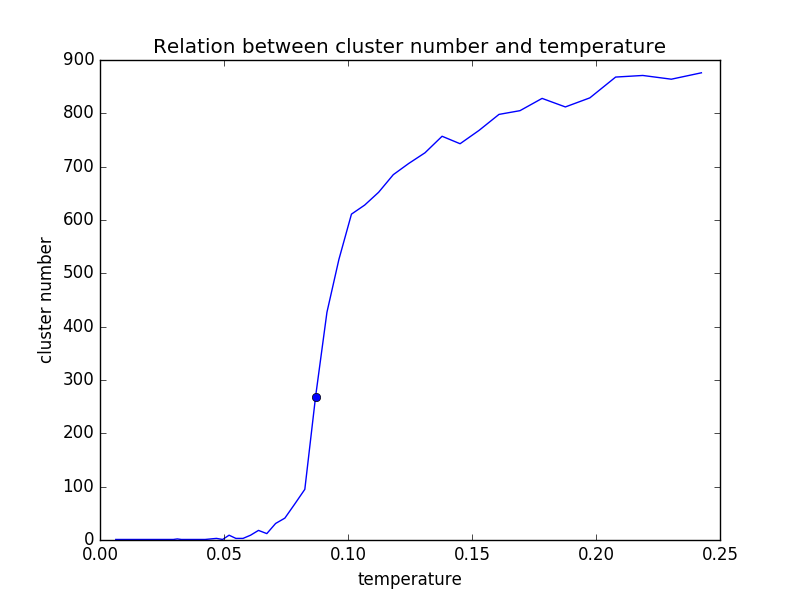
\includegraphics[width=.8\linewidth]{fig/cluster_num.png}
  \caption{}%Relation between the total number of clusters and temperature with the selected temperature $T_{final}$.}
  \label{fig:cluster_num}
\end{subfigure}
\hspace*{\fill}
\begin{subfigure}{0.45\textwidth}
  \centering
  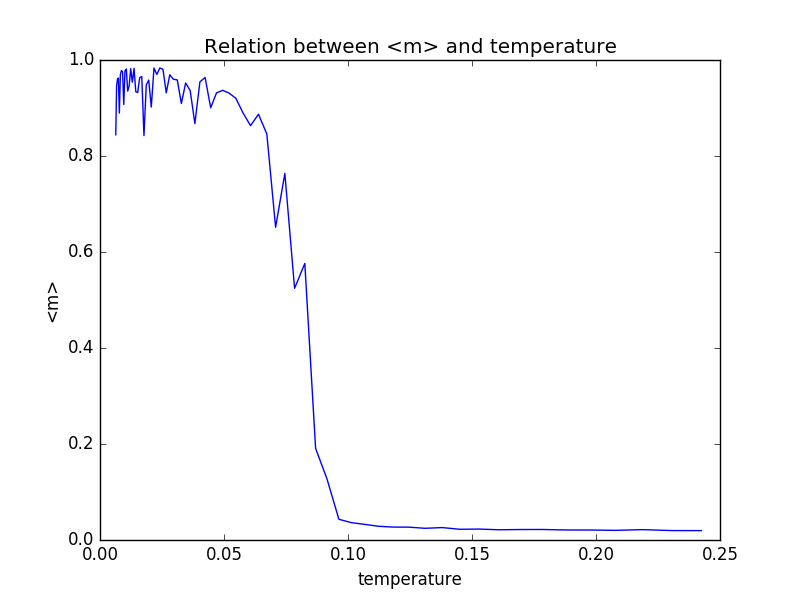
\includegraphics[width=.8\linewidth]{fig/magnetization.png}
  \caption{}%Relation between the magnetization and temperature.}
  \label{fig:magnetization}
\end{subfigure}
\begin{subfigure}{0.45\textwidth}
  \centering
  
  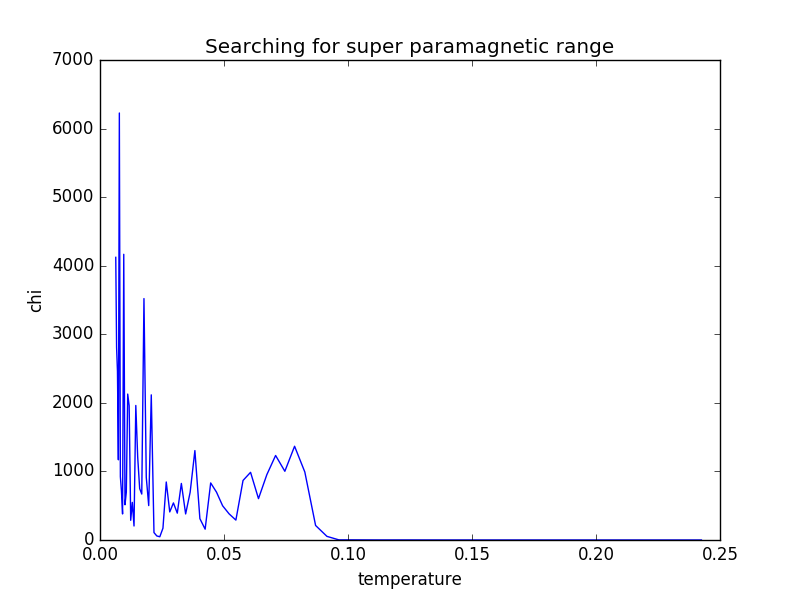
\includegraphics[width=.8\linewidth]{fig/suspencability.png}
  \caption{}%Relation between the susceptibility and temperature.}
  \label{fig:suspenc}
\end{subfigure}
\hspace*{\fill}
\begin{subfigure}{0.45\textwidth}
  \centering
  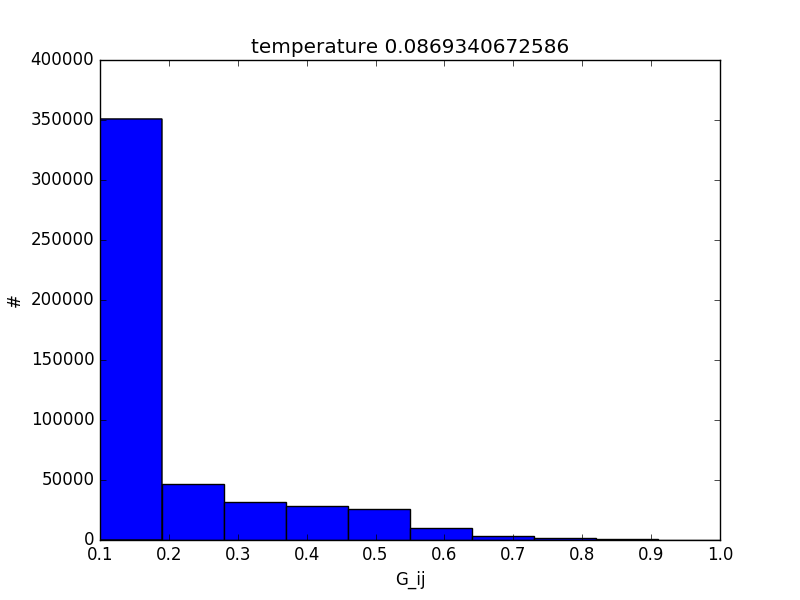
\includegraphics[width=.8\linewidth]{fig/temp__.png}
  \caption{}%Distribution of $G$.}
  \label{fig:gij}
\end{subfigure}
\end{figure}

\end{frame}



\begin{frame}
\frametitle{Results}

\begin{figure}
\begin{subfigure}{0.45\textwidth}
  \centering
  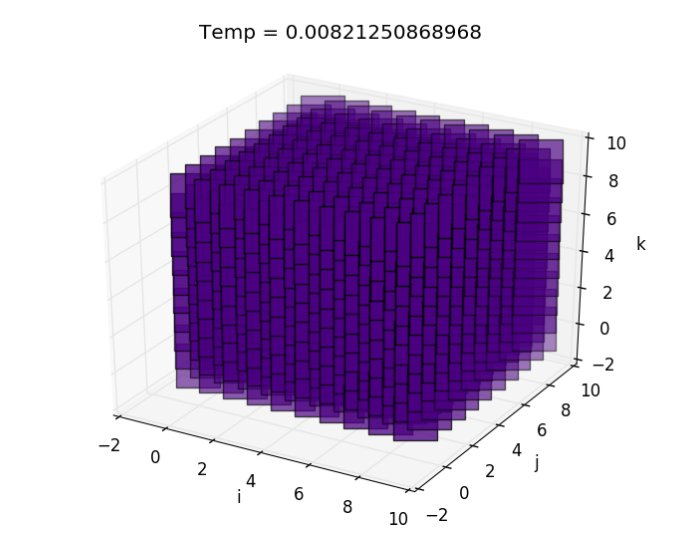
\includegraphics[width=.8\linewidth]{fig/low_temp.jpg}
  \caption{}%L}
  \label{fig:low_tmp}
\end{subfigure}
\hspace*{\fill}
\begin{subfigure}{0.45\textwidth}
  \centering

  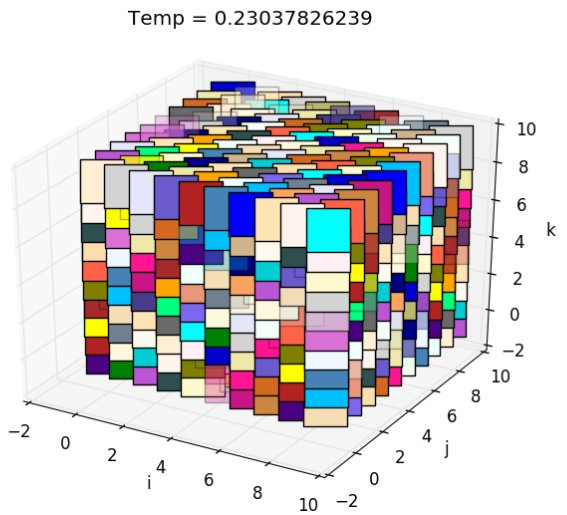
\includegraphics[width=.8\linewidth]{fig/high_tmp.jpg}
  \caption{}%}
  \label{fig:high_temp}
\end{subfigure}

\begin{subfigure}{0.45\textwidth}
  \centering
  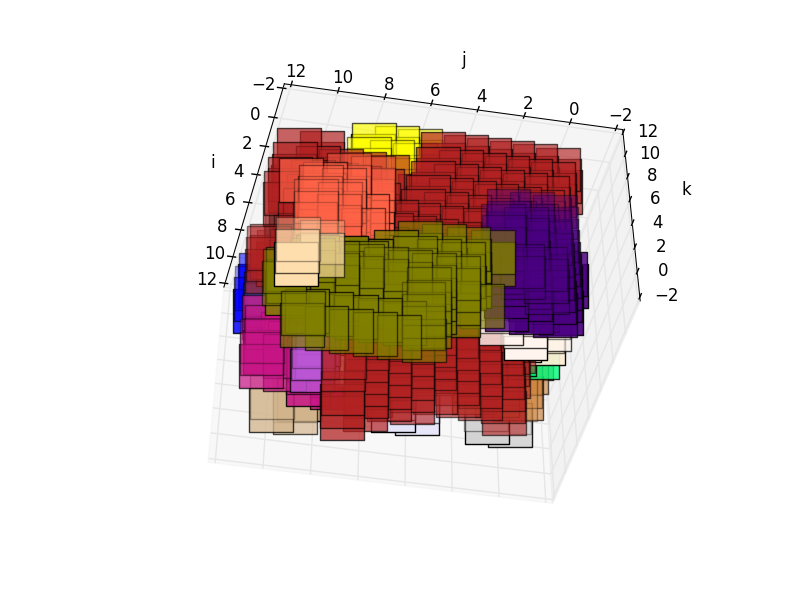
\includegraphics[width=.9\linewidth]{fig/figure_1.png}
  \caption{}%Final clustering result of a (12, 12, 12) voxel grid.}
  \label{fig:fig_good_final_cluster_12}
\end{subfigure}
\hspace*{\fill}
\begin{subfigure}{0.45\textwidth}
  \centering

  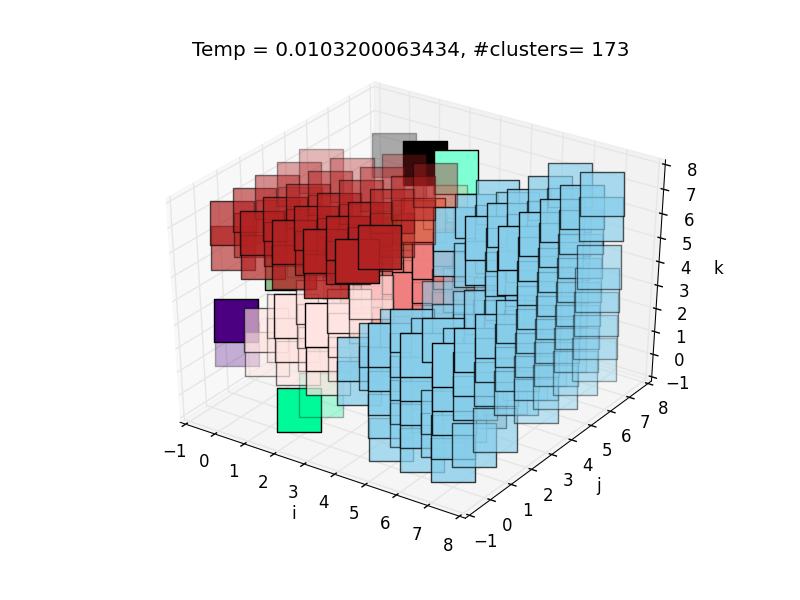
\includegraphics[width=.9\linewidth]{fig/cluster-8x8x8-2.png}
  \caption{}%Final clustering result of a (8, 8, 8) voxel grid.}
  \label{fig:fig_good_final_cluster_7}
\end{subfigure}

\end{figure}
\end{frame}


\begin{frame}
    \frametitle{References}
    
    \printbibliography
\end{frame}

\end{document}

